%\pdfoutput=0
\documentclass[onecolumn]{article}
\usepackage{graphicx}
\usepackage{hyperref}
\usepackage{amsmath}
\usepackage[a4paper,margin=4.75cm,tmargin=3.1cm,bmargin=3.1cm]{geometry}

\title{Exam: Question 11 \\ \large \textbf{Multidimensional pseudo-random (plain Monte Carlo) vs
quasi-random (Halton and/or lattice sequence) integrators}\\
Investigate the convergence rates (of some interesting integrals in
different dimensions) as function of the number of sample points.}
\author{Lukas Martin Wick\\
Student number: 201707977}
\begin{document}


\maketitle
Three Multidimensional Monte Carlo integrators using respectively pseudo-random (plain) and quasi-random Halton and lattice sequences. 
The convergence rate has been tested on different integrals. First a simple test integral is the area of a circle wit radius $r = 1$, and

\begin{align}
   \int^{1.1}_{-1.1} dx \int^{1.1}_{-1.1} dy \rho(x,y) = \pi,
\end{align}
where, 
\begin{align}
\rho(x,y) =
\begin{cases}
    1 & \text{if } x^2+y^2\leq r^2  \\
    0 & \text{else }      %
\end{cases}
\end{align}
The convergence can be seen in Figure \ref{fig:circle}. Here the actual error is the absolute
difference to the exact result, and the estimated error is the methods expected
error. The quasi random integrators use the difference between two runs with
half of the points. In the figure the error of the integrators has been fitted.

A slightly more difficult version integrates the volume of a half sphere, for $r=\left(\frac{3}{2}\right)^(1/3)\approx 1.145$ giving
\begin{align}
    \int^{1.5}_{-1.5} dx \int^{1.5}_{-1.5} dy \rho(x,y) = \pi,
 \end{align}
 where here, 
 \begin{align}
 \rho(x,y) =
 \begin{cases}
     \sqrt{r^2-x^2+y^2} & \text{if } x^2+y^2\leq r^2  \\
     0 & \text{else }      %
 \end{cases}
\end{align}
The convergence of this can be seen in Figure \ref{fig:sphere}.

The convergence for the integral 
\begin{align}
    \int^{\pi}_{0} dx \int^{\pi}_{0} dy \int^{\pi}_{0} dz \sin(x)\sin(y)\sin(z) = 8,
\end{align}
can be seen in Figure \ref{fig:sin}. The convergence for the harder integral 
\begin{align}
    &\frac{1}{\pi^3}\int^{\pi}_{0} dx \int^{\pi}_{0} dy \int^{\pi}_{0} dz \frac{1}{1-\cos(x)\cos(y)\cos(z)}=  \frac{\Gamma\left(\frac{1}{4}\right)^4}{4\pi^3} \\&= 1.3932039296856768591842462603255,
\end{align}
can be seen in Figure \ref{fig:cos}. In all figures the fitted a is given for each method.
It is illustrated that in general, except in the case of the very hard integral, the quasi-random methods dose better 
than the pseudo-random, and that in general the Halton sequence dose slightly better than the lattice sequence, with a small difference. 
The pseudo-random integrator dose converge close to $a=0.5\Rightarrow\text{Error}\sim\frac{1}{\sqrt{N}}$ for the easy problems of the sphere and circle.
The error estimates seen fairly precise, but slightly overestimated, except for in the hard problem

\begin{figure}[h]
    \centering
    \makebox[\textwidth][c]{% GNUPLOT: LaTeX picture with Postscript
\begingroup
  \makeatletter
  \providecommand\color[2][]{%
    \GenericError{(gnuplot) \space\space\space\@spaces}{%
      Package color not loaded in conjunction with
      terminal option `colourtext'%
    }{See the gnuplot documentation for explanation.%
    }{Either use 'blacktext' in gnuplot or load the package
      color.sty in LaTeX.}%
    \renewcommand\color[2][]{}%
  }%
  \providecommand\includegraphics[2][]{%
    \GenericError{(gnuplot) \space\space\space\@spaces}{%
      Package graphicx or graphics not loaded%
    }{See the gnuplot documentation for explanation.%
    }{The gnuplot epslatex terminal needs graphicx.sty or graphics.sty.}%
    \renewcommand\includegraphics[2][]{}%
  }%
  \providecommand\rotatebox[2]{#2}%
  \@ifundefined{ifGPcolor}{%
    \newif\ifGPcolor
    \GPcolortrue
  }{}%
  \@ifundefined{ifGPblacktext}{%
    \newif\ifGPblacktext
    \GPblacktexttrue
  }{}%
  % define a \g@addto@macro without @ in the name:
  \let\gplgaddtomacro\g@addto@macro
  % define empty templates for all commands taking text:
  \gdef\gplbacktext{}%
  \gdef\gplfronttext{}%
  \makeatother
  \ifGPblacktext
    % no textcolor at all
    \def\colorrgb#1{}%
    \def\colorgray#1{}%
  \else
    % gray or color?
    \ifGPcolor
      \def\colorrgb#1{\color[rgb]{#1}}%
      \def\colorgray#1{\color[gray]{#1}}%
      \expandafter\def\csname LTw\endcsname{\color{white}}%
      \expandafter\def\csname LTb\endcsname{\color{black}}%
      \expandafter\def\csname LTa\endcsname{\color{black}}%
      \expandafter\def\csname LT0\endcsname{\color[rgb]{1,0,0}}%
      \expandafter\def\csname LT1\endcsname{\color[rgb]{0,1,0}}%
      \expandafter\def\csname LT2\endcsname{\color[rgb]{0,0,1}}%
      \expandafter\def\csname LT3\endcsname{\color[rgb]{1,0,1}}%
      \expandafter\def\csname LT4\endcsname{\color[rgb]{0,1,1}}%
      \expandafter\def\csname LT5\endcsname{\color[rgb]{1,1,0}}%
      \expandafter\def\csname LT6\endcsname{\color[rgb]{0,0,0}}%
      \expandafter\def\csname LT7\endcsname{\color[rgb]{1,0.3,0}}%
      \expandafter\def\csname LT8\endcsname{\color[rgb]{0.5,0.5,0.5}}%
    \else
      % gray
      \def\colorrgb#1{\color{black}}%
      \def\colorgray#1{\color[gray]{#1}}%
      \expandafter\def\csname LTw\endcsname{\color{white}}%
      \expandafter\def\csname LTb\endcsname{\color{black}}%
      \expandafter\def\csname LTa\endcsname{\color{black}}%
      \expandafter\def\csname LT0\endcsname{\color{black}}%
      \expandafter\def\csname LT1\endcsname{\color{black}}%
      \expandafter\def\csname LT2\endcsname{\color{black}}%
      \expandafter\def\csname LT3\endcsname{\color{black}}%
      \expandafter\def\csname LT4\endcsname{\color{black}}%
      \expandafter\def\csname LT5\endcsname{\color{black}}%
      \expandafter\def\csname LT6\endcsname{\color{black}}%
      \expandafter\def\csname LT7\endcsname{\color{black}}%
      \expandafter\def\csname LT8\endcsname{\color{black}}%
    \fi
  \fi
    \setlength{\unitlength}{0.0500bp}%
    \ifx\gptboxheight\undefined%
      \newlength{\gptboxheight}%
      \newlength{\gptboxwidth}%
      \newsavebox{\gptboxtext}%
    \fi%
    \setlength{\fboxrule}{0.5pt}%
    \setlength{\fboxsep}{1pt}%
\begin{picture}(11520.00,5760.00)%
    \gplgaddtomacro\gplbacktext{%
      \csname LTb\endcsname%
      \put(1155,1025){\makebox(0,0)[r]{\strut{}0.000010}}%
      \csname LTb\endcsname%
      \put(1155,1774){\makebox(0,0)[r]{\strut{}0.000100}}%
      \csname LTb\endcsname%
      \put(1155,2523){\makebox(0,0)[r]{\strut{}0.001000}}%
      \csname LTb\endcsname%
      \put(1155,3273){\makebox(0,0)[r]{\strut{}0.010000}}%
      \csname LTb\endcsname%
      \put(1155,4022){\makebox(0,0)[r]{\strut{}0.100000}}%
      \csname LTb\endcsname%
      \put(1155,4771){\makebox(0,0)[r]{\strut{}1.000000}}%
      \csname LTb\endcsname%
      \put(1257,614){\makebox(0,0){\strut{}$10$}}%
      \csname LTb\endcsname%
      \put(1956,614){\makebox(0,0){\strut{}$100$}}%
      \csname LTb\endcsname%
      \put(2656,614){\makebox(0,0){\strut{}$1000$}}%
      \csname LTb\endcsname%
      \put(3355,614){\makebox(0,0){\strut{}$10000$}}%
      \csname LTb\endcsname%
      \put(4054,614){\makebox(0,0){\strut{}$100000$}}%
      \csname LTb\endcsname%
      \put(4754,614){\makebox(0,0){\strut{}$1\times10^{6}$}}%
      \csname LTb\endcsname%
      \put(5453,614){\makebox(0,0){\strut{}$1\times10^{7}$}}%
    }%
    \gplgaddtomacro\gplfronttext{%
      \csname LTb\endcsname%
      \put(144,2898){\rotatebox{-270}{\makebox(0,0){\strut{}Error}}}%
      \csname LTb\endcsname%
      \put(3355,335){\makebox(0,0){\strut{}N}}%
      \csname LTb\endcsname%
      \put(3355,5275){\makebox(0,0){\strut{}Error}}%
      \csname LTb\endcsname%
      \put(2583,1897){\makebox(0,0)[r]{\strut{}Plain}}%
      \csname LTb\endcsname%
      \put(2583,1711){\makebox(0,0)[r]{\strut{}Halton}}%
      \csname LTb\endcsname%
      \put(2583,1525){\makebox(0,0)[r]{\strut{}Lattice}}%
      \csname LTb\endcsname%
      \put(2583,1339){\makebox(0,0)[r]{\strut{}FitP :a:{0.57}}}%
      \csname LTb\endcsname%
      \put(2583,1153){\makebox(0,0)[r]{\strut{}FitH :a:{0.66}}}%
      \csname LTb\endcsname%
      \put(2583,967){\makebox(0,0)[r]{\strut{}FitL :a:{0.70}}}%
    }%
    \gplgaddtomacro\gplbacktext{%
      \csname LTb\endcsname%
      \put(6915,1025){\makebox(0,0)[r]{\strut{}0.000010}}%
      \csname LTb\endcsname%
      \put(6915,1774){\makebox(0,0)[r]{\strut{}0.000100}}%
      \csname LTb\endcsname%
      \put(6915,2523){\makebox(0,0)[r]{\strut{}0.001000}}%
      \csname LTb\endcsname%
      \put(6915,3273){\makebox(0,0)[r]{\strut{}0.010000}}%
      \csname LTb\endcsname%
      \put(6915,4022){\makebox(0,0)[r]{\strut{}0.100000}}%
      \csname LTb\endcsname%
      \put(6915,4771){\makebox(0,0)[r]{\strut{}1.000000}}%
      \csname LTb\endcsname%
      \put(7017,614){\makebox(0,0){\strut{}$10$}}%
      \csname LTb\endcsname%
      \put(7716,614){\makebox(0,0){\strut{}$100$}}%
      \csname LTb\endcsname%
      \put(8416,614){\makebox(0,0){\strut{}$1000$}}%
      \csname LTb\endcsname%
      \put(9115,614){\makebox(0,0){\strut{}$10000$}}%
      \csname LTb\endcsname%
      \put(9814,614){\makebox(0,0){\strut{}$100000$}}%
      \csname LTb\endcsname%
      \put(10514,614){\makebox(0,0){\strut{}$1\times10^{6}$}}%
      \csname LTb\endcsname%
      \put(11213,614){\makebox(0,0){\strut{}$1\times10^{7}$}}%
    }%
    \gplgaddtomacro\gplfronttext{%
      \csname LTb\endcsname%
      \put(5904,2898){\rotatebox{-270}{\makebox(0,0){\strut{}Error}}}%
      \csname LTb\endcsname%
      \put(9115,335){\makebox(0,0){\strut{}N}}%
      \csname LTb\endcsname%
      \put(9115,5275){\makebox(0,0){\strut{}Estimated Error }}%
      \csname LTb\endcsname%
      \put(7833,1339){\makebox(0,0)[r]{\strut{}Plain}}%
      \csname LTb\endcsname%
      \put(7833,1153){\makebox(0,0)[r]{\strut{}Halton}}%
      \csname LTb\endcsname%
      \put(7833,967){\makebox(0,0)[r]{\strut{}Lattice}}%
    }%
    \gplbacktext
    \put(0,0){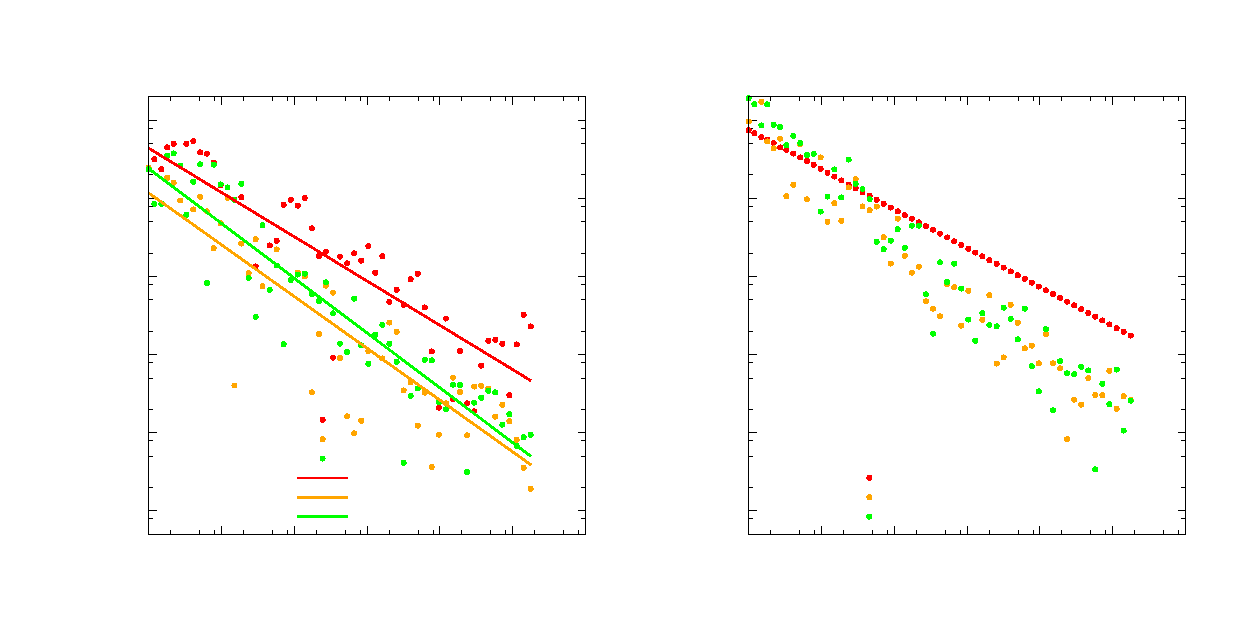
\includegraphics{plotCircle}}%
    \gplfronttext
  \end{picture}%
\endgroup
}
    \caption{Monte carlo convergence rate for the integral of a circle.}
    \label{fig:circle}
\end{figure}
\begin{figure}[h]
    \centering
    \makebox[\textwidth][c]{% GNUPLOT: LaTeX picture with Postscript
\begingroup
  \makeatletter
  \providecommand\color[2][]{%
    \GenericError{(gnuplot) \space\space\space\@spaces}{%
      Package color not loaded in conjunction with
      terminal option `colourtext'%
    }{See the gnuplot documentation for explanation.%
    }{Either use 'blacktext' in gnuplot or load the package
      color.sty in LaTeX.}%
    \renewcommand\color[2][]{}%
  }%
  \providecommand\includegraphics[2][]{%
    \GenericError{(gnuplot) \space\space\space\@spaces}{%
      Package graphicx or graphics not loaded%
    }{See the gnuplot documentation for explanation.%
    }{The gnuplot epslatex terminal needs graphicx.sty or graphics.sty.}%
    \renewcommand\includegraphics[2][]{}%
  }%
  \providecommand\rotatebox[2]{#2}%
  \@ifundefined{ifGPcolor}{%
    \newif\ifGPcolor
    \GPcolortrue
  }{}%
  \@ifundefined{ifGPblacktext}{%
    \newif\ifGPblacktext
    \GPblacktexttrue
  }{}%
  % define a \g@addto@macro without @ in the name:
  \let\gplgaddtomacro\g@addto@macro
  % define empty templates for all commands taking text:
  \gdef\gplbacktext{}%
  \gdef\gplfronttext{}%
  \makeatother
  \ifGPblacktext
    % no textcolor at all
    \def\colorrgb#1{}%
    \def\colorgray#1{}%
  \else
    % gray or color?
    \ifGPcolor
      \def\colorrgb#1{\color[rgb]{#1}}%
      \def\colorgray#1{\color[gray]{#1}}%
      \expandafter\def\csname LTw\endcsname{\color{white}}%
      \expandafter\def\csname LTb\endcsname{\color{black}}%
      \expandafter\def\csname LTa\endcsname{\color{black}}%
      \expandafter\def\csname LT0\endcsname{\color[rgb]{1,0,0}}%
      \expandafter\def\csname LT1\endcsname{\color[rgb]{0,1,0}}%
      \expandafter\def\csname LT2\endcsname{\color[rgb]{0,0,1}}%
      \expandafter\def\csname LT3\endcsname{\color[rgb]{1,0,1}}%
      \expandafter\def\csname LT4\endcsname{\color[rgb]{0,1,1}}%
      \expandafter\def\csname LT5\endcsname{\color[rgb]{1,1,0}}%
      \expandafter\def\csname LT6\endcsname{\color[rgb]{0,0,0}}%
      \expandafter\def\csname LT7\endcsname{\color[rgb]{1,0.3,0}}%
      \expandafter\def\csname LT8\endcsname{\color[rgb]{0.5,0.5,0.5}}%
    \else
      % gray
      \def\colorrgb#1{\color{black}}%
      \def\colorgray#1{\color[gray]{#1}}%
      \expandafter\def\csname LTw\endcsname{\color{white}}%
      \expandafter\def\csname LTb\endcsname{\color{black}}%
      \expandafter\def\csname LTa\endcsname{\color{black}}%
      \expandafter\def\csname LT0\endcsname{\color{black}}%
      \expandafter\def\csname LT1\endcsname{\color{black}}%
      \expandafter\def\csname LT2\endcsname{\color{black}}%
      \expandafter\def\csname LT3\endcsname{\color{black}}%
      \expandafter\def\csname LT4\endcsname{\color{black}}%
      \expandafter\def\csname LT5\endcsname{\color{black}}%
      \expandafter\def\csname LT6\endcsname{\color{black}}%
      \expandafter\def\csname LT7\endcsname{\color{black}}%
      \expandafter\def\csname LT8\endcsname{\color{black}}%
    \fi
  \fi
    \setlength{\unitlength}{0.0500bp}%
    \ifx\gptboxheight\undefined%
      \newlength{\gptboxheight}%
      \newlength{\gptboxwidth}%
      \newsavebox{\gptboxtext}%
    \fi%
    \setlength{\fboxrule}{0.5pt}%
    \setlength{\fboxsep}{1pt}%
\begin{picture}(11520.00,5760.00)%
    \gplgaddtomacro\gplbacktext{%
      \csname LTb\endcsname%
      \put(1155,1025){\makebox(0,0)[r]{\strut{}0.000010}}%
      \csname LTb\endcsname%
      \put(1155,1774){\makebox(0,0)[r]{\strut{}0.000100}}%
      \csname LTb\endcsname%
      \put(1155,2523){\makebox(0,0)[r]{\strut{}0.001000}}%
      \csname LTb\endcsname%
      \put(1155,3273){\makebox(0,0)[r]{\strut{}0.010000}}%
      \csname LTb\endcsname%
      \put(1155,4022){\makebox(0,0)[r]{\strut{}0.100000}}%
      \csname LTb\endcsname%
      \put(1155,4771){\makebox(0,0)[r]{\strut{}1.000000}}%
      \csname LTb\endcsname%
      \put(1257,614){\makebox(0,0){\strut{}$10$}}%
      \csname LTb\endcsname%
      \put(1956,614){\makebox(0,0){\strut{}$100$}}%
      \csname LTb\endcsname%
      \put(2656,614){\makebox(0,0){\strut{}$1000$}}%
      \csname LTb\endcsname%
      \put(3355,614){\makebox(0,0){\strut{}$10000$}}%
      \csname LTb\endcsname%
      \put(4054,614){\makebox(0,0){\strut{}$100000$}}%
      \csname LTb\endcsname%
      \put(4754,614){\makebox(0,0){\strut{}$1\times10^{6}$}}%
      \csname LTb\endcsname%
      \put(5453,614){\makebox(0,0){\strut{}$1\times10^{7}$}}%
    }%
    \gplgaddtomacro\gplfronttext{%
      \csname LTb\endcsname%
      \put(144,2898){\rotatebox{-270}{\makebox(0,0){\strut{}Error}}}%
      \csname LTb\endcsname%
      \put(3355,335){\makebox(0,0){\strut{}N}}%
      \csname LTb\endcsname%
      \put(3355,5275){\makebox(0,0){\strut{}Error}}%
      \csname LTb\endcsname%
      \put(2583,1897){\makebox(0,0)[r]{\strut{}Plain}}%
      \csname LTb\endcsname%
      \put(2583,1711){\makebox(0,0)[r]{\strut{}Halton}}%
      \csname LTb\endcsname%
      \put(2583,1525){\makebox(0,0)[r]{\strut{}Lattice}}%
      \csname LTb\endcsname%
      \put(2583,1339){\makebox(0,0)[r]{\strut{}FitP :a:{0.46}}}%
      \csname LTb\endcsname%
      \put(2583,1153){\makebox(0,0)[r]{\strut{}FitH :a:{0.99}}}%
      \csname LTb\endcsname%
      \put(2583,967){\makebox(0,0)[r]{\strut{}FitL :a:{1.00}}}%
    }%
    \gplgaddtomacro\gplbacktext{%
      \csname LTb\endcsname%
      \put(6915,1025){\makebox(0,0)[r]{\strut{}0.000010}}%
      \csname LTb\endcsname%
      \put(6915,1774){\makebox(0,0)[r]{\strut{}0.000100}}%
      \csname LTb\endcsname%
      \put(6915,2523){\makebox(0,0)[r]{\strut{}0.001000}}%
      \csname LTb\endcsname%
      \put(6915,3273){\makebox(0,0)[r]{\strut{}0.010000}}%
      \csname LTb\endcsname%
      \put(6915,4022){\makebox(0,0)[r]{\strut{}0.100000}}%
      \csname LTb\endcsname%
      \put(6915,4771){\makebox(0,0)[r]{\strut{}1.000000}}%
      \csname LTb\endcsname%
      \put(7017,614){\makebox(0,0){\strut{}$10$}}%
      \csname LTb\endcsname%
      \put(7716,614){\makebox(0,0){\strut{}$100$}}%
      \csname LTb\endcsname%
      \put(8416,614){\makebox(0,0){\strut{}$1000$}}%
      \csname LTb\endcsname%
      \put(9115,614){\makebox(0,0){\strut{}$10000$}}%
      \csname LTb\endcsname%
      \put(9814,614){\makebox(0,0){\strut{}$100000$}}%
      \csname LTb\endcsname%
      \put(10514,614){\makebox(0,0){\strut{}$1\times10^{6}$}}%
      \csname LTb\endcsname%
      \put(11213,614){\makebox(0,0){\strut{}$1\times10^{7}$}}%
    }%
    \gplgaddtomacro\gplfronttext{%
      \csname LTb\endcsname%
      \put(5904,2898){\rotatebox{-270}{\makebox(0,0){\strut{}Error}}}%
      \csname LTb\endcsname%
      \put(9115,335){\makebox(0,0){\strut{}N}}%
      \csname LTb\endcsname%
      \put(9115,5275){\makebox(0,0){\strut{}Estimated Error }}%
      \csname LTb\endcsname%
      \put(7833,1339){\makebox(0,0)[r]{\strut{}Plain}}%
      \csname LTb\endcsname%
      \put(7833,1153){\makebox(0,0)[r]{\strut{}Halton}}%
      \csname LTb\endcsname%
      \put(7833,967){\makebox(0,0)[r]{\strut{}Lattice}}%
    }%
    \gplbacktext
    \put(0,0){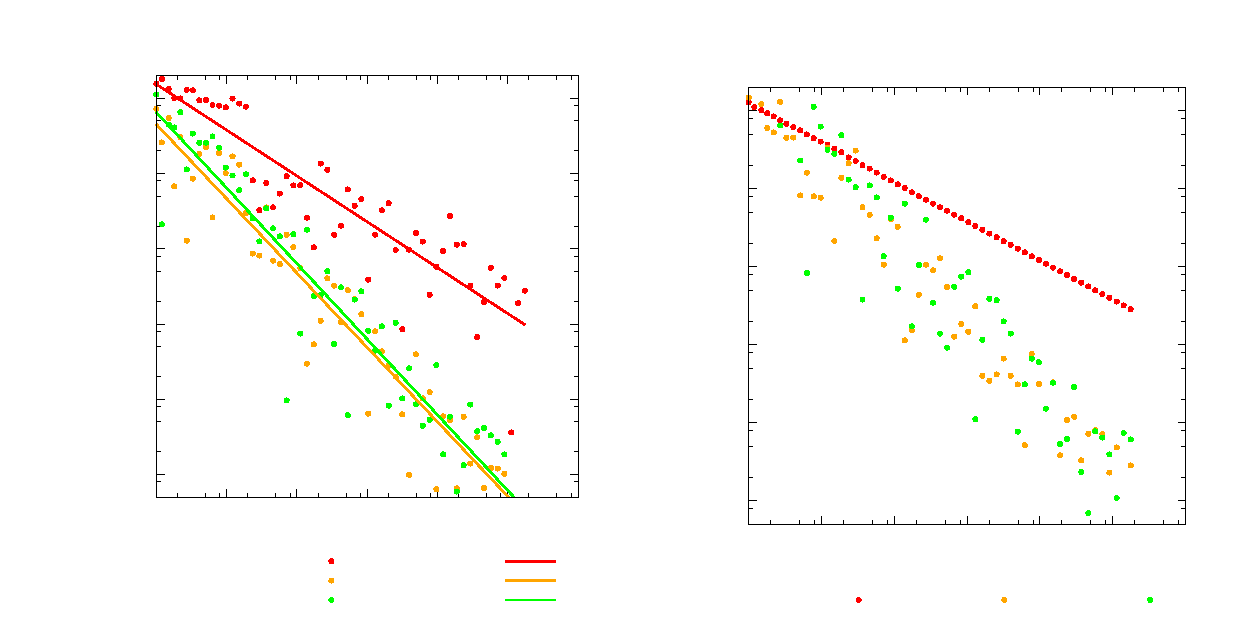
\includegraphics{plotSphere}}%
    \gplfronttext
  \end{picture}%
\endgroup
}
    \caption{Monte carlo convergence rate for the integral of a half sphere.}
    \label{fig:sphere}
\end{figure}
\begin{figure}[h]
    \centering
    \makebox[\textwidth][c]{% GNUPLOT: LaTeX picture with Postscript
\begingroup
  \makeatletter
  \providecommand\color[2][]{%
    \GenericError{(gnuplot) \space\space\space\@spaces}{%
      Package color not loaded in conjunction with
      terminal option `colourtext'%
    }{See the gnuplot documentation for explanation.%
    }{Either use 'blacktext' in gnuplot or load the package
      color.sty in LaTeX.}%
    \renewcommand\color[2][]{}%
  }%
  \providecommand\includegraphics[2][]{%
    \GenericError{(gnuplot) \space\space\space\@spaces}{%
      Package graphicx or graphics not loaded%
    }{See the gnuplot documentation for explanation.%
    }{The gnuplot epslatex terminal needs graphicx.sty or graphics.sty.}%
    \renewcommand\includegraphics[2][]{}%
  }%
  \providecommand\rotatebox[2]{#2}%
  \@ifundefined{ifGPcolor}{%
    \newif\ifGPcolor
    \GPcolortrue
  }{}%
  \@ifundefined{ifGPblacktext}{%
    \newif\ifGPblacktext
    \GPblacktexttrue
  }{}%
  % define a \g@addto@macro without @ in the name:
  \let\gplgaddtomacro\g@addto@macro
  % define empty templates for all commands taking text:
  \gdef\gplbacktext{}%
  \gdef\gplfronttext{}%
  \makeatother
  \ifGPblacktext
    % no textcolor at all
    \def\colorrgb#1{}%
    \def\colorgray#1{}%
  \else
    % gray or color?
    \ifGPcolor
      \def\colorrgb#1{\color[rgb]{#1}}%
      \def\colorgray#1{\color[gray]{#1}}%
      \expandafter\def\csname LTw\endcsname{\color{white}}%
      \expandafter\def\csname LTb\endcsname{\color{black}}%
      \expandafter\def\csname LTa\endcsname{\color{black}}%
      \expandafter\def\csname LT0\endcsname{\color[rgb]{1,0,0}}%
      \expandafter\def\csname LT1\endcsname{\color[rgb]{0,1,0}}%
      \expandafter\def\csname LT2\endcsname{\color[rgb]{0,0,1}}%
      \expandafter\def\csname LT3\endcsname{\color[rgb]{1,0,1}}%
      \expandafter\def\csname LT4\endcsname{\color[rgb]{0,1,1}}%
      \expandafter\def\csname LT5\endcsname{\color[rgb]{1,1,0}}%
      \expandafter\def\csname LT6\endcsname{\color[rgb]{0,0,0}}%
      \expandafter\def\csname LT7\endcsname{\color[rgb]{1,0.3,0}}%
      \expandafter\def\csname LT8\endcsname{\color[rgb]{0.5,0.5,0.5}}%
    \else
      % gray
      \def\colorrgb#1{\color{black}}%
      \def\colorgray#1{\color[gray]{#1}}%
      \expandafter\def\csname LTw\endcsname{\color{white}}%
      \expandafter\def\csname LTb\endcsname{\color{black}}%
      \expandafter\def\csname LTa\endcsname{\color{black}}%
      \expandafter\def\csname LT0\endcsname{\color{black}}%
      \expandafter\def\csname LT1\endcsname{\color{black}}%
      \expandafter\def\csname LT2\endcsname{\color{black}}%
      \expandafter\def\csname LT3\endcsname{\color{black}}%
      \expandafter\def\csname LT4\endcsname{\color{black}}%
      \expandafter\def\csname LT5\endcsname{\color{black}}%
      \expandafter\def\csname LT6\endcsname{\color{black}}%
      \expandafter\def\csname LT7\endcsname{\color{black}}%
      \expandafter\def\csname LT8\endcsname{\color{black}}%
    \fi
  \fi
    \setlength{\unitlength}{0.0500bp}%
    \ifx\gptboxheight\undefined%
      \newlength{\gptboxheight}%
      \newlength{\gptboxwidth}%
      \newsavebox{\gptboxtext}%
    \fi%
    \setlength{\fboxrule}{0.5pt}%
    \setlength{\fboxsep}{1pt}%
\begin{picture}(11520.00,5760.00)%
    \gplgaddtomacro\gplbacktext{%
      \csname LTb\endcsname%
      \put(1155,1025){\makebox(0,0)[r]{\strut{}0.000010}}%
      \csname LTb\endcsname%
      \put(1155,1774){\makebox(0,0)[r]{\strut{}0.000100}}%
      \csname LTb\endcsname%
      \put(1155,2523){\makebox(0,0)[r]{\strut{}0.001000}}%
      \csname LTb\endcsname%
      \put(1155,3273){\makebox(0,0)[r]{\strut{}0.010000}}%
      \csname LTb\endcsname%
      \put(1155,4022){\makebox(0,0)[r]{\strut{}0.100000}}%
      \csname LTb\endcsname%
      \put(1155,4771){\makebox(0,0)[r]{\strut{}1.000000}}%
      \csname LTb\endcsname%
      \put(1257,614){\makebox(0,0){\strut{}$10$}}%
      \csname LTb\endcsname%
      \put(1956,614){\makebox(0,0){\strut{}$100$}}%
      \csname LTb\endcsname%
      \put(2656,614){\makebox(0,0){\strut{}$1000$}}%
      \csname LTb\endcsname%
      \put(3355,614){\makebox(0,0){\strut{}$10000$}}%
      \csname LTb\endcsname%
      \put(4054,614){\makebox(0,0){\strut{}$100000$}}%
      \csname LTb\endcsname%
      \put(4754,614){\makebox(0,0){\strut{}$1\times10^{6}$}}%
      \csname LTb\endcsname%
      \put(5453,614){\makebox(0,0){\strut{}$1\times10^{7}$}}%
    }%
    \gplgaddtomacro\gplfronttext{%
      \csname LTb\endcsname%
      \put(144,2898){\rotatebox{-270}{\makebox(0,0){\strut{}Error}}}%
      \csname LTb\endcsname%
      \put(3355,335){\makebox(0,0){\strut{}N}}%
      \csname LTb\endcsname%
      \put(3355,5275){\makebox(0,0){\strut{}Error}}%
      \csname LTb\endcsname%
      \put(2583,1897){\makebox(0,0)[r]{\strut{}Plain}}%
      \csname LTb\endcsname%
      \put(2583,1711){\makebox(0,0)[r]{\strut{}Halton}}%
      \csname LTb\endcsname%
      \put(2583,1525){\makebox(0,0)[r]{\strut{}Lattice}}%
      \csname LTb\endcsname%
      \put(2583,1339){\makebox(0,0)[r]{\strut{}FitP :a:{0.38}}}%
      \csname LTb\endcsname%
      \put(2583,1153){\makebox(0,0)[r]{\strut{}FitH :a:{0.99}}}%
      \csname LTb\endcsname%
      \put(2583,967){\makebox(0,0)[r]{\strut{}FitL :a:{0.96}}}%
    }%
    \gplgaddtomacro\gplbacktext{%
      \csname LTb\endcsname%
      \put(6915,1025){\makebox(0,0)[r]{\strut{}0.000010}}%
      \csname LTb\endcsname%
      \put(6915,1774){\makebox(0,0)[r]{\strut{}0.000100}}%
      \csname LTb\endcsname%
      \put(6915,2523){\makebox(0,0)[r]{\strut{}0.001000}}%
      \csname LTb\endcsname%
      \put(6915,3273){\makebox(0,0)[r]{\strut{}0.010000}}%
      \csname LTb\endcsname%
      \put(6915,4022){\makebox(0,0)[r]{\strut{}0.100000}}%
      \csname LTb\endcsname%
      \put(6915,4771){\makebox(0,0)[r]{\strut{}1.000000}}%
      \csname LTb\endcsname%
      \put(7017,614){\makebox(0,0){\strut{}$10$}}%
      \csname LTb\endcsname%
      \put(7716,614){\makebox(0,0){\strut{}$100$}}%
      \csname LTb\endcsname%
      \put(8416,614){\makebox(0,0){\strut{}$1000$}}%
      \csname LTb\endcsname%
      \put(9115,614){\makebox(0,0){\strut{}$10000$}}%
      \csname LTb\endcsname%
      \put(9814,614){\makebox(0,0){\strut{}$100000$}}%
      \csname LTb\endcsname%
      \put(10514,614){\makebox(0,0){\strut{}$1\times10^{6}$}}%
      \csname LTb\endcsname%
      \put(11213,614){\makebox(0,0){\strut{}$1\times10^{7}$}}%
    }%
    \gplgaddtomacro\gplfronttext{%
      \csname LTb\endcsname%
      \put(5904,2898){\rotatebox{-270}{\makebox(0,0){\strut{}Error}}}%
      \csname LTb\endcsname%
      \put(9115,335){\makebox(0,0){\strut{}N}}%
      \csname LTb\endcsname%
      \put(9115,5275){\makebox(0,0){\strut{}Estimated Error }}%
      \csname LTb\endcsname%
      \put(7833,1339){\makebox(0,0)[r]{\strut{}Plain}}%
      \csname LTb\endcsname%
      \put(7833,1153){\makebox(0,0)[r]{\strut{}Halton}}%
      \csname LTb\endcsname%
      \put(7833,967){\makebox(0,0)[r]{\strut{}Lattice}}%
    }%
    \gplbacktext
    \put(0,0){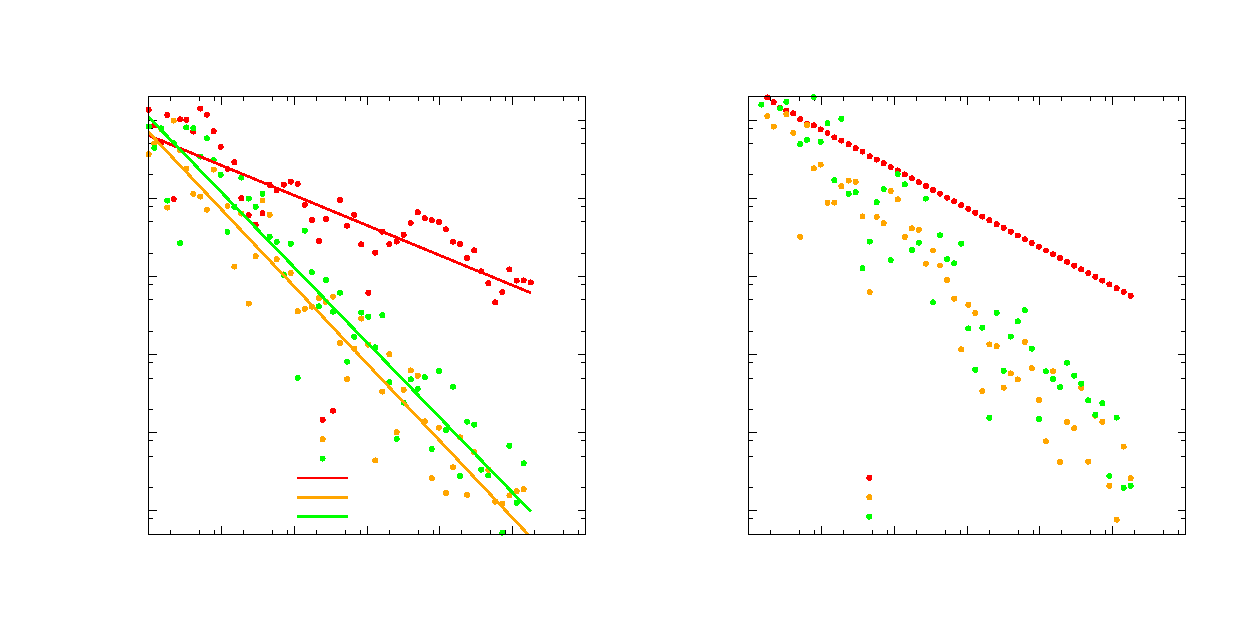
\includegraphics{plotSin}}%
    \gplfronttext
  \end{picture}%
\endgroup
}
    \caption{Monte carlo convergence rates for the integral of $\sin(x)\sin(y)\sin(z)$.}
    \label{fig:sin}
\end{figure}
\begin{figure}[h]
    \centering
    \makebox[\textwidth][c]{% GNUPLOT: LaTeX picture with Postscript
\begingroup
  \makeatletter
  \providecommand\color[2][]{%
    \GenericError{(gnuplot) \space\space\space\@spaces}{%
      Package color not loaded in conjunction with
      terminal option `colourtext'%
    }{See the gnuplot documentation for explanation.%
    }{Either use 'blacktext' in gnuplot or load the package
      color.sty in LaTeX.}%
    \renewcommand\color[2][]{}%
  }%
  \providecommand\includegraphics[2][]{%
    \GenericError{(gnuplot) \space\space\space\@spaces}{%
      Package graphicx or graphics not loaded%
    }{See the gnuplot documentation for explanation.%
    }{The gnuplot epslatex terminal needs graphicx.sty or graphics.sty.}%
    \renewcommand\includegraphics[2][]{}%
  }%
  \providecommand\rotatebox[2]{#2}%
  \@ifundefined{ifGPcolor}{%
    \newif\ifGPcolor
    \GPcolortrue
  }{}%
  \@ifundefined{ifGPblacktext}{%
    \newif\ifGPblacktext
    \GPblacktexttrue
  }{}%
  % define a \g@addto@macro without @ in the name:
  \let\gplgaddtomacro\g@addto@macro
  % define empty templates for all commands taking text:
  \gdef\gplbacktext{}%
  \gdef\gplfronttext{}%
  \makeatother
  \ifGPblacktext
    % no textcolor at all
    \def\colorrgb#1{}%
    \def\colorgray#1{}%
  \else
    % gray or color?
    \ifGPcolor
      \def\colorrgb#1{\color[rgb]{#1}}%
      \def\colorgray#1{\color[gray]{#1}}%
      \expandafter\def\csname LTw\endcsname{\color{white}}%
      \expandafter\def\csname LTb\endcsname{\color{black}}%
      \expandafter\def\csname LTa\endcsname{\color{black}}%
      \expandafter\def\csname LT0\endcsname{\color[rgb]{1,0,0}}%
      \expandafter\def\csname LT1\endcsname{\color[rgb]{0,1,0}}%
      \expandafter\def\csname LT2\endcsname{\color[rgb]{0,0,1}}%
      \expandafter\def\csname LT3\endcsname{\color[rgb]{1,0,1}}%
      \expandafter\def\csname LT4\endcsname{\color[rgb]{0,1,1}}%
      \expandafter\def\csname LT5\endcsname{\color[rgb]{1,1,0}}%
      \expandafter\def\csname LT6\endcsname{\color[rgb]{0,0,0}}%
      \expandafter\def\csname LT7\endcsname{\color[rgb]{1,0.3,0}}%
      \expandafter\def\csname LT8\endcsname{\color[rgb]{0.5,0.5,0.5}}%
    \else
      % gray
      \def\colorrgb#1{\color{black}}%
      \def\colorgray#1{\color[gray]{#1}}%
      \expandafter\def\csname LTw\endcsname{\color{white}}%
      \expandafter\def\csname LTb\endcsname{\color{black}}%
      \expandafter\def\csname LTa\endcsname{\color{black}}%
      \expandafter\def\csname LT0\endcsname{\color{black}}%
      \expandafter\def\csname LT1\endcsname{\color{black}}%
      \expandafter\def\csname LT2\endcsname{\color{black}}%
      \expandafter\def\csname LT3\endcsname{\color{black}}%
      \expandafter\def\csname LT4\endcsname{\color{black}}%
      \expandafter\def\csname LT5\endcsname{\color{black}}%
      \expandafter\def\csname LT6\endcsname{\color{black}}%
      \expandafter\def\csname LT7\endcsname{\color{black}}%
      \expandafter\def\csname LT8\endcsname{\color{black}}%
    \fi
  \fi
    \setlength{\unitlength}{0.0500bp}%
    \ifx\gptboxheight\undefined%
      \newlength{\gptboxheight}%
      \newlength{\gptboxwidth}%
      \newsavebox{\gptboxtext}%
    \fi%
    \setlength{\fboxrule}{0.5pt}%
    \setlength{\fboxsep}{1pt}%
\begin{picture}(11520.00,5760.00)%
    \gplgaddtomacro\gplbacktext{%
      \csname LTb\endcsname%
      \put(1155,1025){\makebox(0,0)[r]{\strut{}0.000010}}%
      \csname LTb\endcsname%
      \put(1155,1774){\makebox(0,0)[r]{\strut{}0.000100}}%
      \csname LTb\endcsname%
      \put(1155,2523){\makebox(0,0)[r]{\strut{}0.001000}}%
      \csname LTb\endcsname%
      \put(1155,3273){\makebox(0,0)[r]{\strut{}0.010000}}%
      \csname LTb\endcsname%
      \put(1155,4022){\makebox(0,0)[r]{\strut{}0.100000}}%
      \csname LTb\endcsname%
      \put(1155,4771){\makebox(0,0)[r]{\strut{}1.000000}}%
      \csname LTb\endcsname%
      \put(1257,614){\makebox(0,0){\strut{}$10$}}%
      \csname LTb\endcsname%
      \put(1956,614){\makebox(0,0){\strut{}$100$}}%
      \csname LTb\endcsname%
      \put(2656,614){\makebox(0,0){\strut{}$1000$}}%
      \csname LTb\endcsname%
      \put(3355,614){\makebox(0,0){\strut{}$10000$}}%
      \csname LTb\endcsname%
      \put(4054,614){\makebox(0,0){\strut{}$100000$}}%
      \csname LTb\endcsname%
      \put(4754,614){\makebox(0,0){\strut{}$1\times10^{6}$}}%
      \csname LTb\endcsname%
      \put(5453,614){\makebox(0,0){\strut{}$1\times10^{7}$}}%
    }%
    \gplgaddtomacro\gplfronttext{%
      \csname LTb\endcsname%
      \put(144,2898){\rotatebox{-270}{\makebox(0,0){\strut{}Error}}}%
      \csname LTb\endcsname%
      \put(3355,335){\makebox(0,0){\strut{}N}}%
      \csname LTb\endcsname%
      \put(3355,5275){\makebox(0,0){\strut{}Error}}%
      \csname LTb\endcsname%
      \put(2583,1897){\makebox(0,0)[r]{\strut{}Plain}}%
      \csname LTb\endcsname%
      \put(2583,1711){\makebox(0,0)[r]{\strut{}Halton}}%
      \csname LTb\endcsname%
      \put(2583,1525){\makebox(0,0)[r]{\strut{}Lattice}}%
      \csname LTb\endcsname%
      \put(2583,1339){\makebox(0,0)[r]{\strut{}FitP :a:{0.15}}}%
      \csname LTb\endcsname%
      \put(2583,1153){\makebox(0,0)[r]{\strut{}FitH :a:{0.40}}}%
      \csname LTb\endcsname%
      \put(2583,967){\makebox(0,0)[r]{\strut{}FitL :a:{0.25}}}%
    }%
    \gplgaddtomacro\gplbacktext{%
      \csname LTb\endcsname%
      \put(6915,1025){\makebox(0,0)[r]{\strut{}0.000010}}%
      \csname LTb\endcsname%
      \put(6915,1774){\makebox(0,0)[r]{\strut{}0.000100}}%
      \csname LTb\endcsname%
      \put(6915,2523){\makebox(0,0)[r]{\strut{}0.001000}}%
      \csname LTb\endcsname%
      \put(6915,3273){\makebox(0,0)[r]{\strut{}0.010000}}%
      \csname LTb\endcsname%
      \put(6915,4022){\makebox(0,0)[r]{\strut{}0.100000}}%
      \csname LTb\endcsname%
      \put(6915,4771){\makebox(0,0)[r]{\strut{}1.000000}}%
      \csname LTb\endcsname%
      \put(7017,614){\makebox(0,0){\strut{}$10$}}%
      \csname LTb\endcsname%
      \put(7716,614){\makebox(0,0){\strut{}$100$}}%
      \csname LTb\endcsname%
      \put(8416,614){\makebox(0,0){\strut{}$1000$}}%
      \csname LTb\endcsname%
      \put(9115,614){\makebox(0,0){\strut{}$10000$}}%
      \csname LTb\endcsname%
      \put(9814,614){\makebox(0,0){\strut{}$100000$}}%
      \csname LTb\endcsname%
      \put(10514,614){\makebox(0,0){\strut{}$1\times10^{6}$}}%
      \csname LTb\endcsname%
      \put(11213,614){\makebox(0,0){\strut{}$1\times10^{7}$}}%
    }%
    \gplgaddtomacro\gplfronttext{%
      \csname LTb\endcsname%
      \put(5904,2898){\rotatebox{-270}{\makebox(0,0){\strut{}Error}}}%
      \csname LTb\endcsname%
      \put(9115,335){\makebox(0,0){\strut{}N}}%
      \csname LTb\endcsname%
      \put(9115,5275){\makebox(0,0){\strut{}Estimated Error }}%
      \csname LTb\endcsname%
      \put(7833,1339){\makebox(0,0)[r]{\strut{}Plain}}%
      \csname LTb\endcsname%
      \put(7833,1153){\makebox(0,0)[r]{\strut{}Halton}}%
      \csname LTb\endcsname%
      \put(7833,967){\makebox(0,0)[r]{\strut{}Lattice}}%
    }%
    \gplbacktext
    \put(0,0){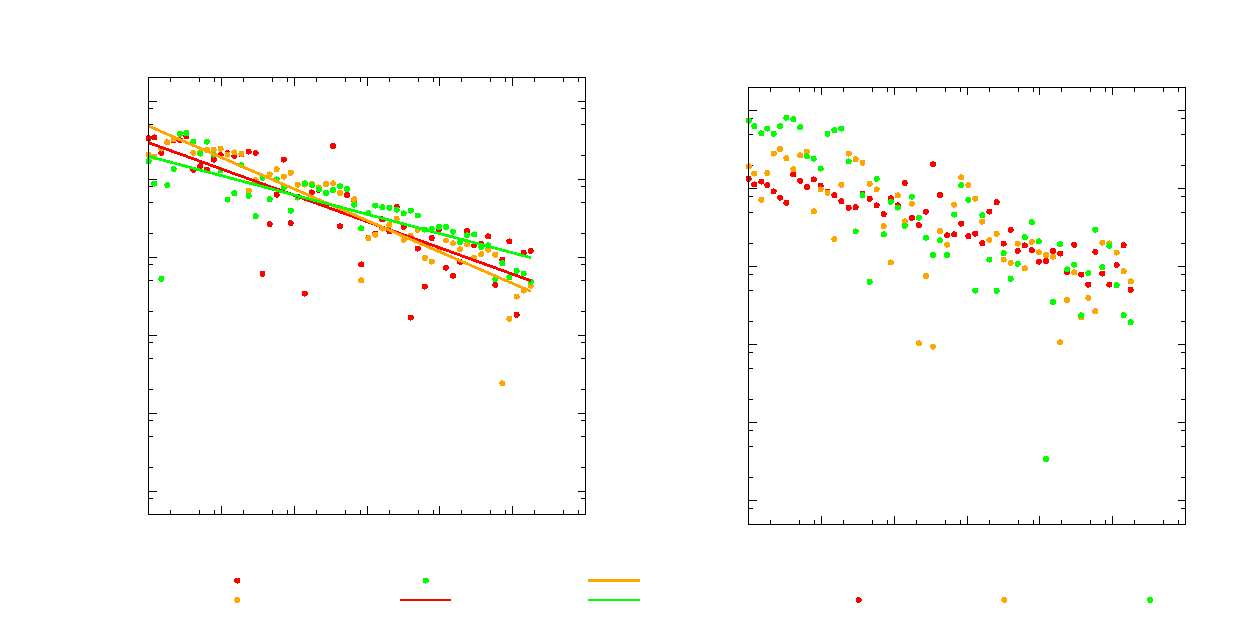
\includegraphics{plotHard}}%
    \gplfronttext
  \end{picture}%
\endgroup
}
    \caption{Monte carlo convergence rates for the integral of $\frac{1}{1-\cos(x)\cos(y)\cos(z)}$.}
    \label{fig:cos}
\end{figure}

\end{document}
